\subsection{Umgang mit dem Kompass}
Generelle Feindsichtungen nach R-E-Z (Richtung-Entfernung-Ziel) Prinzip \\

Gut geeignet für schnelle Ausrichtung im Gelände. Simple Information über mögliche Kontakte, besonders wenn man verteilt steht.
\begin{figure}[!h]
	\centering
	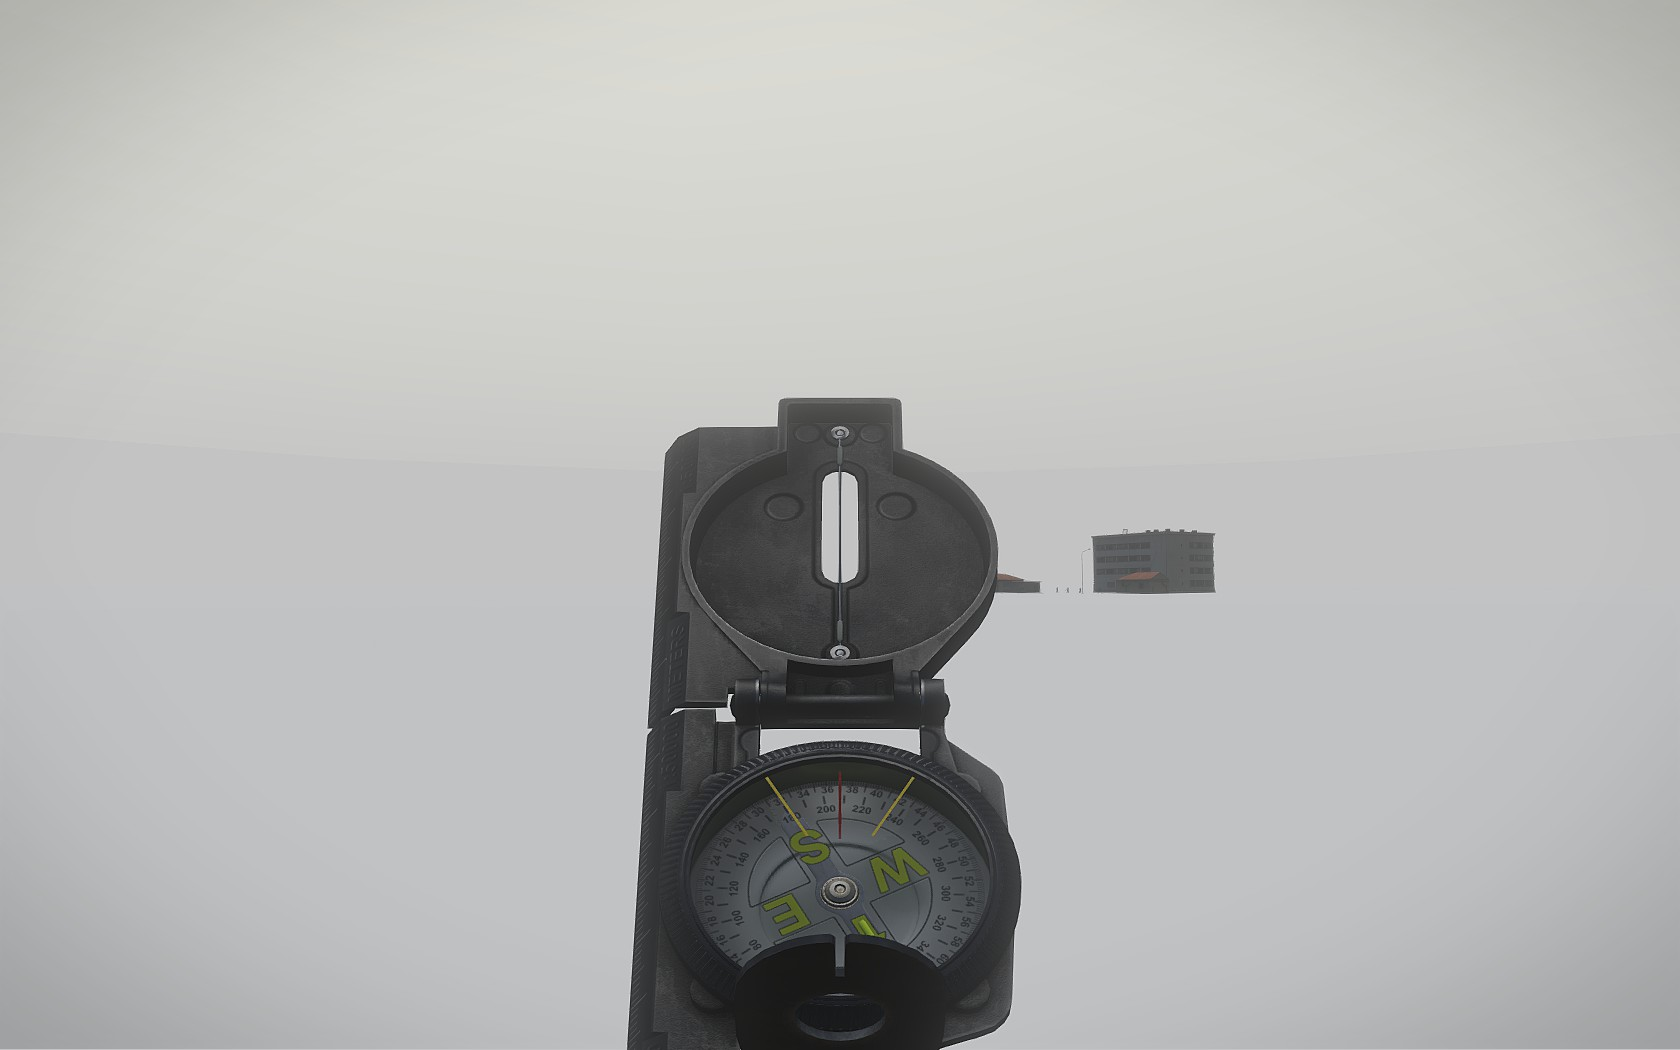
\includegraphics[width=0.7\textwidth]{./img/fortgeschrittenes/karteUndMarkierungen/Kompass1.jpg}
	\caption{Beispiel: Sichtung 4er Infanterie Patrouille in Stadtgebiet}
\end{figure}\\
	
Für Zieleinweisung
\begin{itemize}
	\item Ziel mit Feldstecher lokalisieren, mit dem Fadenkreuz anpeilen.
	\item Ohne sich zu bewegen auf den Kompass Wechseln für die genaue Gradzahl bzw. Ausrichtung des Kompassdrahts an markanten Stellen oder auf den Feind, sofern Sichtbar.
\end{itemize}

\begin{figure}[!h]
	\centering
	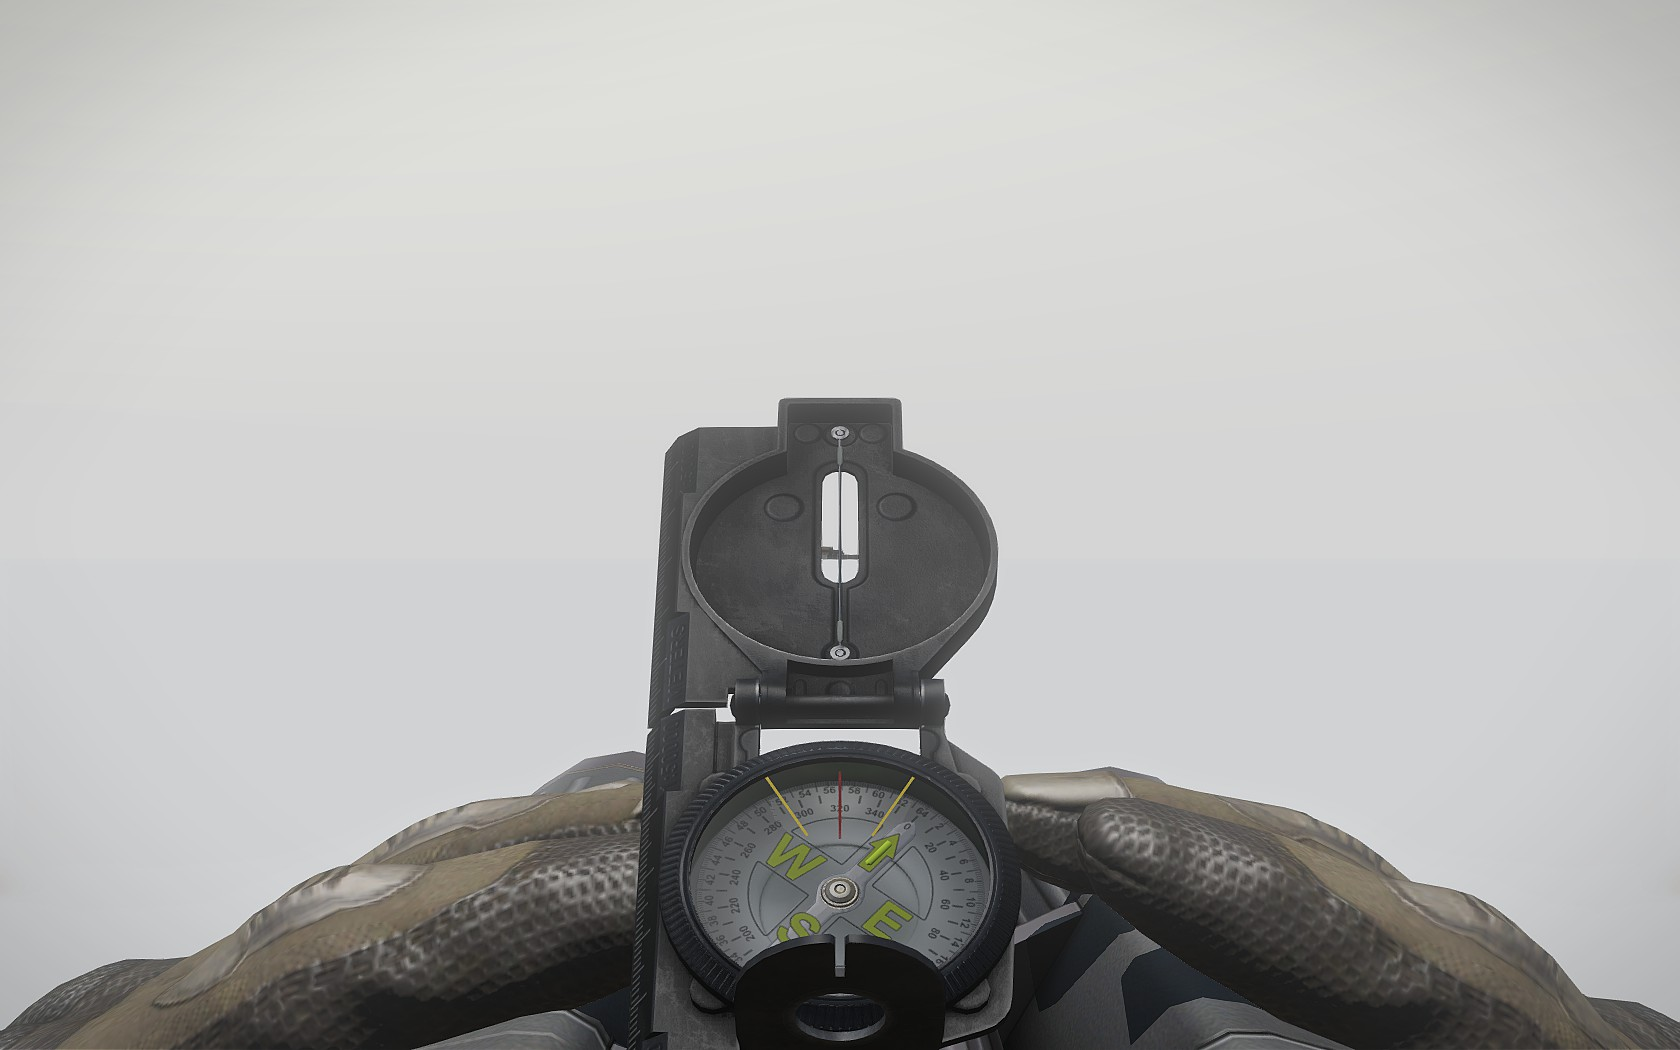
\includegraphics[width=0.75\textwidth]{./img/fortgeschrittenes/karteUndMarkierungen/Kompass2.jpg}
\end{figure}

Angabe: >>Kontakt im Südwesten 300 m, links vom hohen Bürogebäude, 4 Mann Patroullie, kalt<< (Bitte beachten das weitere Informationen hilfreich sein können z.B. Art der Bewaffnung)\\

Feindsichtungen nach Gradzahlen
Gut geeignet für eindeutige Bestimmung von Feinden für Gruppenscharfschützen und Fahrzeuge, die entweder dicht bei euch stehen oder in einer Linie hinter mit eurer Position stehen. Auch sehr nützlich für die präzisere Kartenmarkierung von Feinden.
\begin{figure}[!h]
	\centering
	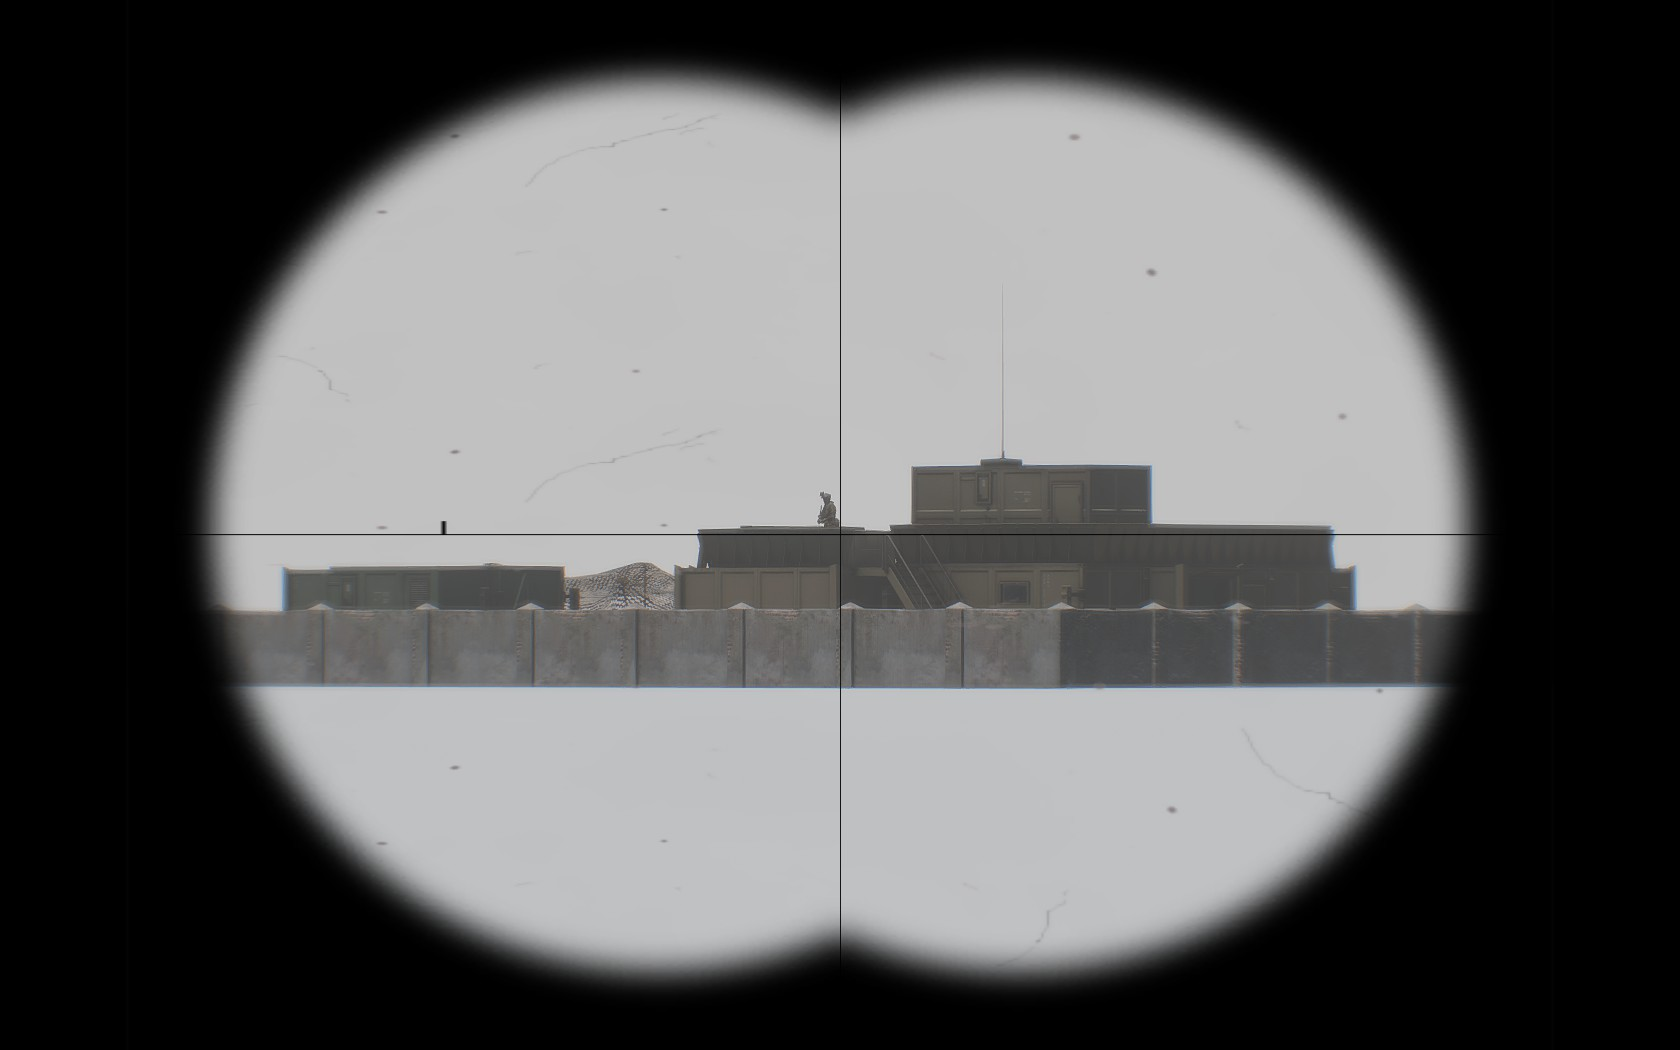
\includegraphics[width=0.75\textwidth]{./img/fortgeschrittenes/karteUndMarkierungen/Kompass3.jpg}
	\caption{Situation: Einzelner feindlicher Kontakt auf HQ Gebäude}
\end{figure}\\

Für Zieleinweisung
\begin{itemize}
	\item Ziel mit Feldstecher lokalisieren, mit dem Fadenkreuz anpeilen.
	\item Ohne sich zu bewegen auf den Kompass Wechseln für die genaue Gradzahl bzw. Ausrichtung des Kompassdrahts an markanten Stellen oder auf den Feind, sofern Sichtbar.
\end{itemize}

\begin{figure}[!h]
	\centering
	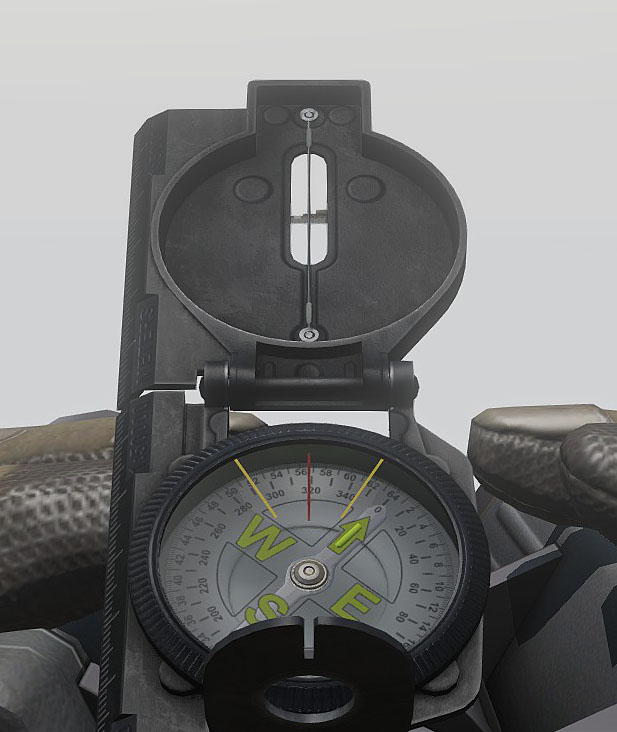
\includegraphics[width=0.65\textwidth]{./img/fortgeschrittenes/karteUndMarkierungen/Kompass4.jpg}
\end{figure}
Angabe: >>Kontakt NW, 319° von meiner Position, 500m, einzelner Schütze auf dem Militärgebäude, kalt.<<\\

Feindsichtungen mit MILS (Strich / Artilleriepromille) \\

Hierbei werden die natürlichen Gradzahlen in einem Volkreis mit 6400 Einheiten aufgeteilt, was die Zieleinweisung bei über 1000m einen Seitenabstand des Ziels von einem Meter ergibt. Diese befinden sich auf dem 3., äusseren Zahlenring des Kompasses.\\
Gut geeignet bei sehr weiten Entfernungen 900m+, wo der Winkel der Gradzahlen sehr stark zusammenläuft um sehr exakte Anweisungen für Scharfschützen zu geben bzw. für Mörser / Artillerie Einweisung. Geht nicht ohne dass man direkt nebeneinander steht oder dies entsprechend der Position der Artillerie umrechnet.  \\

\begin{figure}[!h]
	\centering
	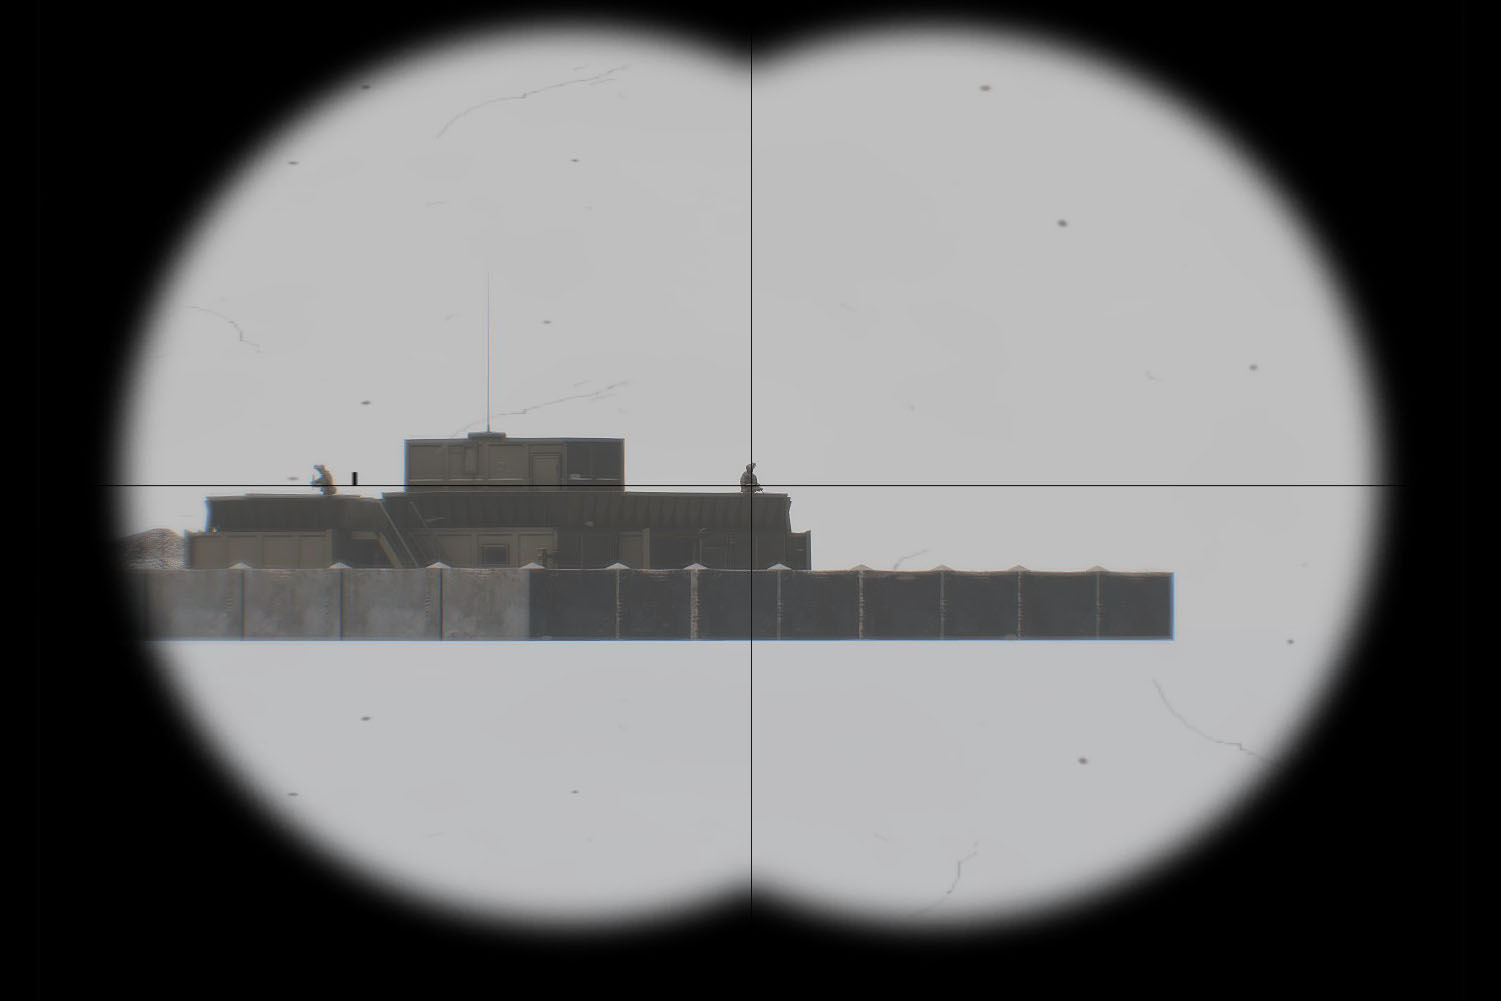
\includegraphics[width=0.75\textwidth]{./img/fortgeschrittenes/karteUndMarkierungen/Kompass5.jpg}
\end{figure}
Situation 2 Infanterieposten auf einem HQ Gebäude. Nur der Rechte soll von unserem Scharfschützen ausgeschaltet werden.\\
\begin{itemize}
 	\item Mit Feldstecher anvisieren.
	\item Ohne sich zu bewegen den Kompass rausholen und im äussersten Zahlenringen ablesen (Gradzahl ist bei rechtem oder linken Pfosten beides 320°) . Hierfür sollte man exakt hinter oder direkt neben dem Schützen positioniert sein.
	\end{itemize}
\begin{figure}[!h]
	\centering
	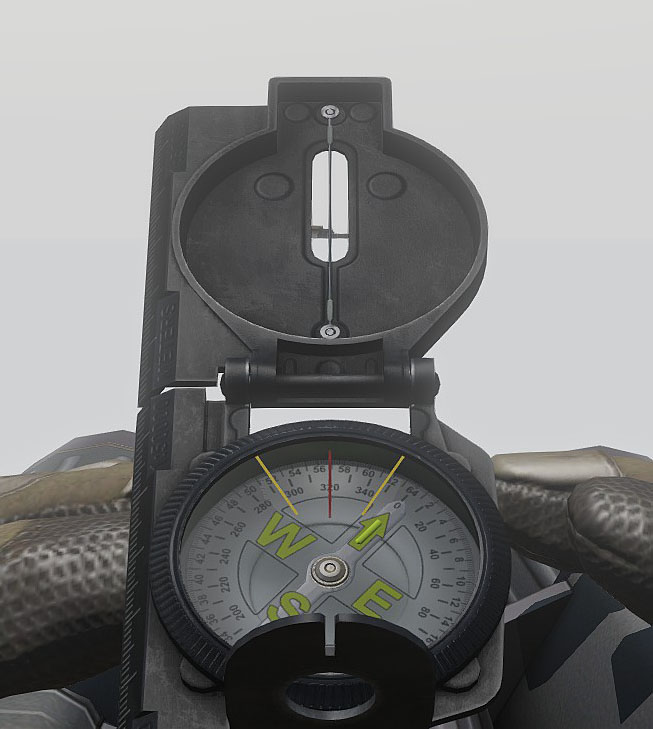
\includegraphics[width=0.65\textwidth]{./img/fortgeschrittenes/karteUndMarkierungen/Kompass6.jpg}
	\caption{>>Kontakt auf 320° meiner Position, 900 m, Strich 5690 , einzelner Schütze, kalt<<}
\end{figure}
